% Yvonnick Esnault - yvonnick.e@free.fr 
% Gaetan Le Brun - gaetan.lebrun@gmail.com
% Thibaut Leli�vre - thibaut.lelievre@voila.fr
% Vincent Mah� - vmahe@free.fr
% Les chapitres peuvent commencer sur une page paire ou impaire
%openany
\documentclass[a4paper,11pt]{article}
%\frontmatter

\usepackage[T1]{fontenc}
\usepackage{ae,aecompl}
\usepackage[frenchb]{babel}
\usepackage[pdftex]{graphicx}
\usepackage[french]{minitoc}
\usepackage{fancyhdr}
\usepackage{lastpage}
\usepackage{hyperref}
\usepackage{textcomp}
%\usepackage [applemac] {inputenc} % les accents
\usepackage{verbatim}
\usepackage{float}

\evensidemargin=13pt
\oddsidemargin=13pt
\topmargin=-\headheight \advance\topmargin by -\headsep
\textwidth=14.59cm \textheight=21.62cm % normal A4, 1'' margin % 24.62cm
\setlength{\parindent}{8mm} % on remet le retrait de paragraphe

%%% My Vars %%%
\def\mytitle{TetraHead}
\def\mysubject{Synth\'etiseur}
\def\mydate{\today}
\def\myversion{1.0}
\def\me{\small  Yvonnick Esnault - Ga�tan Le Brun - Thibaut Leli�vre - Vincent Mah�}
\def\meandmail{\me \\{\normalsize\tt \mymail}}

%%% Fancy headers to add logo, line \ldots{} %%%
\pagestyle{fancy}
\fancyhf{}

% red�finition du style plain pour les pages sp�ciales (chapter)
\fancypagestyle{plain}{
 \fancyhead{}
 \renewcommand{\headrulewidth}{0pt}
 \renewcommand{\footrulewidth}{0.4pt}
 \lfoot{\textsl{\me\space} \\
\mysubject}
 \cfoot{}
 \rfoot{\textsl{Page \thepage \space sur \pageref{LastPage} }}
}

\renewcommand{\headsep}{50pt}

%\renewcommand{\chaptermark}[1]{\markboth{#1}{}}
\renewcommand{\sectionmark}[1]{\markright{#1}}
%\lhead[\thepage]{\rightmark}
%\rhead[\leftmark]{\thepage}

% Header
%\lhead{\includegraphics[width=2cm]{../document_type/images/logo.png}}
\chead{\mysubject} %\leftmark : contient le nom du chapitre courant.
%\rhead{\includegraphics[width=2cm]{images/logo_itin.png}}

%Footer
\lfoot{\textsl{\me\space}}
\cfoot{}
\rfoot{\textsl{Page \thepage \space sur \pageref{LastPage} }}

%Affiche les ligne en haut, et en bas
\renewcommand{\headrulewidth}{0.4pt}
\renewcommand{\footrulewidth}{0.4pt}

%%% bookmarks, linking in pdf %%%
\hypersetup{pdfauthor={\me},%
            pdftitle={\mytitle},%
            pdfsubject={\mysubject},%
            colorlinks,%
            citecolor=black,%
            filecolor=black,%
            linkcolor=black,%
            urlcolor=black,%
            pdftex}

%%% Commande pour supprimer en-t�tes
%%% et pied de page des pages vides
\newcommand{\clearemptydoublepage}{%
\newpage{\pagestyle{empty}\cleardoublepage}}

%%% Environnement pour le tableau de l'historique
\newenvironment{historique}
{

\begin{center}
{\huge \textbf{Historique}}

\vspace{3cm}
\begin{tabular}{|l|l|l|l|}
\hline
\textbf{Date} & \textbf{Auteur} & \textbf{Modifications} & \textbf{Version} \\
\hline
}
{
\end{tabular}\end{center}
\newpage
}

\newcommand{\histo}[4]
{#1 & #2 & #3 & #4 \\
\hline
}


%\newcommand{\info}[1]{
%\begin{figure}
%  \framebox[\textwidth][l]{
%   \begin{minipage}[c]{0.1\textwidth}
%     \medskip
%
%      
\includegraphics{../document_type/images/info.png}
%      \medskip
%
%   \end{minipage} \hfill
%   \begin{minipage}[c]{0.8\textwidth}
%     \medskip
%
%     #1\medskip
%
%   \end{minipage} \hfill
%   \begin{minipage}[c]{0.1\textwidth}
%     \makebox[30pt]{}\par
%   \end{minipage}
%}
%\end{figure}
%}

\newcommand{\encadre}[2]{
\begin{figure}[!h]
  \framebox[\textwidth][l]{
   \begin{minipage}[c]{0.1\textwidth}
     \medskip

      \includegraphics{#1}
      \medskip

   \end{minipage} \hfill
   \begin{minipage}[c]{0.8\textwidth}
     \medskip

     #2\medskip

   \end{minipage} \hfill
   \begin{minipage}[c]{0.1\textwidth}
     \makebox[30pt]{}\par
   \end{minipage}
}
\end{figure}
}

\newcommand{\info}[1]{
\encadre{../document_type/images/info.png}{#1}
}

\newcommand{\attention}[1]{
\encadre{../document_type/images/attention.png}{#1}
}

\newcommand{\code}[1]{\texttt{#1}}

\newcommand{\subsubsubsection}[1]{\textbf{#1}
\medskip

}


\newcommand{\titre}{Algorithmes pour enveloppes}

\newcommand{\diffusion}{Libre & Restreint & \textbf{Confidentiel}}
\newcommand{\etat}{En progression}
\newcommand{\version}{1.0}
\newcommand{\datedoc}{23/01/2006}

\begin{document}

%\frontmatter

%\pagenumbering{Arabic}

\newlength{\larg}
\setlength{\larg}{14.5cm}

\begin{titlepage}

\begin{center}

\includegraphics{../document_type/images/logo_TetraHead_small.png}\\
\end{center}
 
 %\vspace{5.5cm}
 \vspace{\stretch{1}}

{\rule{\larg}{1mm}}\vspace{7mm}
\begin{center}
  {\Huge {\bf {TetraHead - Synth\'etiseur}}} \\
  \medskip
  {\huge \titre}
\end{center}

\vspace{2mm}

{\rule{\larg}{1mm}}
\vspace{2mm} \\
\begin{tabular}{p{11cm} r}
   & {\large \bf 2006}% \\
%   & {\large  \today}
\end{tabular}\\
%\vspace{3cm}
\vspace{\stretch{1}}

\medskip

\begin{center}
\begin{tabular}{|l|l|l|l|}
\hline
\textbf{Diffusion} & \diffusion \\
\hline
�tat & \multicolumn{3}{|l|}{\textbf{\etat}} \\
\hline
Version & \multicolumn{3}{|l|}{\textbf{\version}} \\
\hline
Date & \multicolumn{3}{|l|}{\textbf{\datedoc}} \\
\hline
\end{tabular}

\end{center}

\end{titlepage}



%mainmatter

\begin{historique}
 %\histo{Date}{Pr�nom Nom}{Modification}{Version}
 \histo{31/01/2006}{Vincent MAH�}{Cr�ation}{1.0}
\end{historique}

\section{Description}
Ce document collecte les diff�rents algorithmes d'enveloppes pour le projet. Chaque algorithme est trait� dans une section distincte.
Il contient :
\begin{itemize}
 \item un court descriptif de l'algorithme
 \item l'origine de l'algorithme
 \item les explications �ventuelles
 \item un exemple de codage de l'algorithme
\end{itemize}

\section{G�n�ralit�s}

\textbf{ADSR envelope}

\smallskip
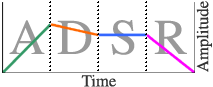
\includegraphics{Adsr_graph.png}
\smallskip

\begin{quote}
\emph{From Wikipedia, the free encyclopedia.}

An ADSR envelope is a parameter used in synthesizers, including those that produce sound by subtractive synthesis, to control the sound produced.

When a mechanical musical instrument produces sound, the relative volume of the sound produced changes over time. The way that this varies is different from instrument to instrument. For instance, a pipe organ, when a key is pressed, plays a note at constant volume, the sound ending virtually as soon as the key is released. The sound of a guitar, by contrast, is loudest immediately after it is played, and fades with time. Other instruments have their own characteristic volume patterns. The ADSR envelope is a way to specify the appropriate behaviour for a "voice" created by the synthesizer. Although usually applied to volume, it is also common to control other sound elements such as filter frequencies or oscillator pitches via ADSR envelope.

The ADSR envelope is specified using four parameters:

Attack 
    How quickly the sound reaches full volume after the sound is activated (the key is pressed). For most mechanical instruments, this period is virtually instantaneous. However, some for some popular synthesized "voices" that don't mimic real instruments, this parameter is slowed down.
Decay 
    How quickly the sound reduces in volume after the initial peak.
Sustain 
    The "constant" volume that the sound takes after decay until the note is released. Note that this parameter specifies a volume level rather than a time period.
Release 
    How quickly the sound fades after the end of the note (the key is released). Often, this time is very short. An example where the release is longer might be a percussion instrument like a glockenspiel, or a piano with the sustain pedal pressed.

While ADSR envelopes are a useful first approximation to the volumes of real instruments, they are not a complete substitute. Woodwind and brass instruments give the player the ability to vary the sound arbitrarily throughout a note, for instance. Many synthesizers therefore offer more flexible facilities for volume control that can be used if desired.

On older synthesizers, such as the Korg MS-20, a common variation on the ADSR was ADSHR (attack, decay, sustain, hold, release). By adding a "hold" parameter, the system allowed notes to be held at the sustain level for a length of time before decaying. The General Instruments AY-3-8912 sound chip included the hold time only, the volume level of sustain not being programmable. Another common variation in the same vein is the AHDSR (attack, hold, decay, sustain, release) envelope, in which the "hold" parameter controls how long the envelope stays at full volume before entering the decay phase.
\end{quote}

\section{Module ADHSR}

Le module a cinq param�tres de r�glage :
\begin{itemize}
 \item S : volume choisi pour la phase de suspension, pouvant prendre une valeur entre 0 et le maximum (1).
 \item A : dur�e de l'attaque, en ``secondes'', le volume allant de 0 au maximum.
 \item D : dur�e de la descente, en ``secondes'', depuis le volume maximum (1) jusqu'au volume choisi pour la suspension (S).
 \item H : dur�e de la suspension (Hold), en ``secondes'', avec maintien du volume choisi (S).
 \item R : dur�e de la retomb�e, en ``secondes'', le volume passant du niveau choisi pour la suspension au niveau 0.
\end{itemize}

\section{Trigger et Gate}

Des explications tr�s d�taill�es d'une enveloppe ADSR avec Gate et Trigger, sur le site \url{http://www.musicfromouterspace.com/analogsynth/ADSR001/ADSR001.html}
\smallskip

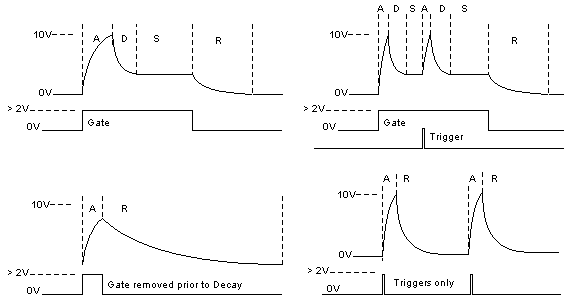
\includegraphics[scale=0.7]{ADSR001_cyclediags.png}
\smallskip

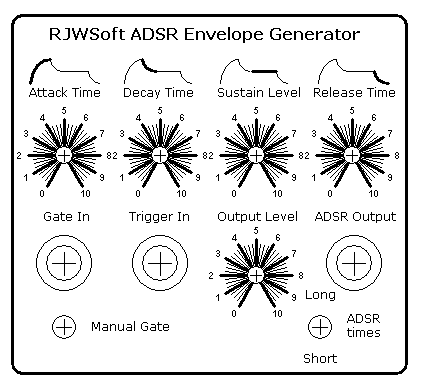
\includegraphics[scale=0.7]{ADSR001_panelsuggestion.png}
\smallskip

\begin{quote}
\textbf{ADSR Envelope Generator (+/-12V or +/-15V)}
\smallskip

Article by Ray Wilson

Features :
\begin{itemize}
 \item 1 mS to 20 second Attack, Decay, and Release times.
 \item Classic ADSR envelope shape and functionality.
 \item Gate and trigger inputs permit retrigger after Attack complete.
 \item Comparators on gate and trigger inputs.
 \item Power Supply Range +/-9V up to +/-15V
\end{itemize}
\medskip

\emph{Introduction}
\smallskip

Envelope generators provide a source of voltage that is shaped like a common amplitude envelope. The gate input is used to initiate the ADSR envelope. The following assumes the gate is maintained throughout the attack, decay and sustain cycles. The voltage envelope rises from 0V to 10 volts during the attack cycle at the rate set by the Attack control. At the peak of the attack cycle (10 volts) the decay cycle is entered. The voltage decays to the sustain level (0 to 10 volts dependant on the setting of the Sustain control) at the rate determined by the Decay control. When the gate is released the release cycle is entered and the voltage decays to 0 at the rate determined by the Release control setting. If the gate is removed at any time during the A,D or S cycle the release state is immediately entered. The trigger input used alone can initiate an attack release cycle. When used in conjunction with the gate the trigger can re-initiate an attack cycle when it occurs during the decay or sustain cycles.
\smallskip

This is an intermediate to advanced project and I do not recommend it as a first project if you are just getting started in synths or electronics. Only the circuit and some explanation are shown here. A lot of project building experience and electronics knowledge and equipment ownership (scope, meters, etc.) is taken for granted. If you are interested in building this project please read the entire page before ordering PC boards to ensure that the information provided is thorough enough for you to complete the project successfully. 
\end{quote}

\end{document}
